\section{模板参数中的编码表达式}

解决这个问题的关键是,在整个表达式之前(示例中,调用赋值操作符之前)不要尝试计算表达式。在求值之前,必须记录哪些操作应用于哪些对象。操作在编译时确定,因此可以对模板参数进行编码。

我们的示例表达式,

\begin{cpp}
1.2*x + x*y;
\end{cpp}

1.2*x的结果不是一个新数组,而是一个表示x的每个值乘以1.2的对象。类似地,x*y必须得到x中的每个元素乘以y中每个对应的元素。当需要得到结果数组的值时,进行存储以备后续的计算。

这里设计一个具体的实现,实现对表达式进行求值

\begin{cpp}
1.2*x + x*y;
\end{cpp}

转换成以下类型的对象:

\begin{cpp}
A_Add<A_Mult<A_Scalar<double>,Array<double>>,
	  A_Mult<Array<double>,Array<double>>>
\end{cpp}

我们将新的基本数组类模板与类模板A\_Scalar、A\_Add和A\_Mult组合在一起。表达式对应的语法树中,可以找到一个前缀表示(参见图27.1)。这个嵌套的模板标识表示所涉及的操作,以及操作应该应用到的对象的类型。A\_Scalar稍后会出现,但其只是数组表达式中标量的占位符。

\begin{center}
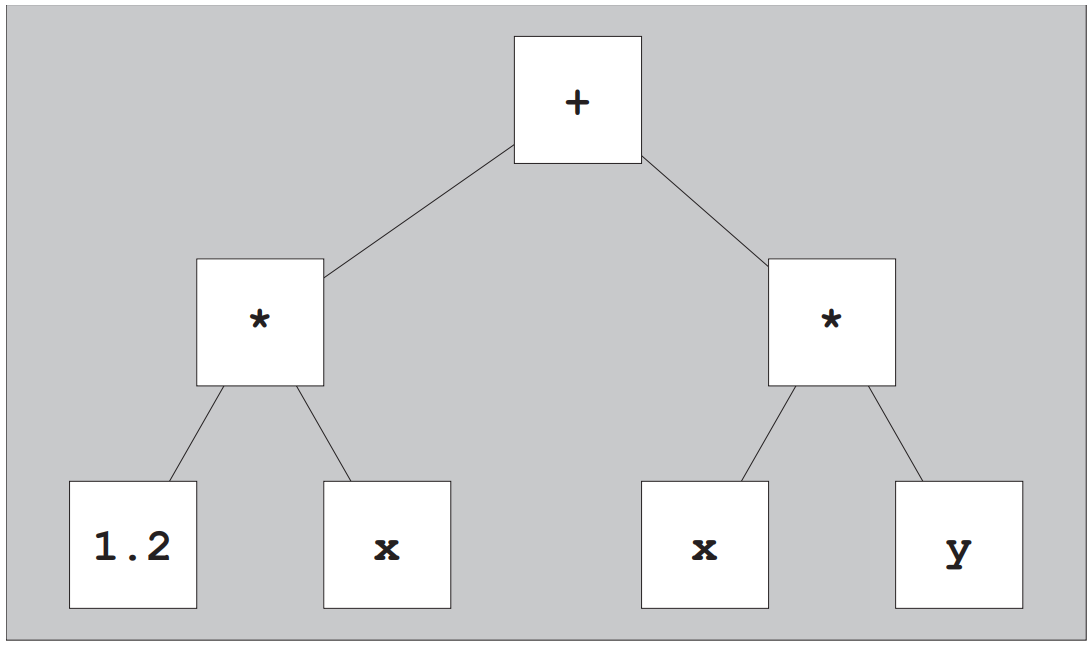
\includegraphics[width=0.6\textwidth]{part3/ch27/images/1.png} \\
图27.1. 表达式1.2*x+x*y的树型表示
\end{center}

\subsection{表达式模板的操作数}

为了完成表达式的表示,必须在每个A\_Add和A\_Mult对象中存储对参数的引用,并记录A\_Scalar对象的值(或对其的引用)。以下是相应操作数的定义:

\filename{exprtmpl/exprops1.hpp}
\begin{cpp}
#include <cstddef>
#include <cassert>

// include helper class traits template to select whether to refer to an
// expression template node either by value or by reference
#include "exprops1a.hpp"

// class for objects that represent the addition of two operands
template<typename T, typename OP1, typename OP2>
class A_Add {
	private:
	typename A_Traits<OP1>::ExprRef op1; // first operand
	typename A_Traits<OP2>::ExprRef op2; // second operand
	
	public:
	// constructor initializes references to operands
	A_Add (OP1 const& a, OP2 const& b)
	: op1(a), op2(b) {
	}

	// compute sum when value requested
	T operator[] (std::size_t idx) const {
		return op1[idx] + op2[idx];
	}

	// size is maximum size
	std::size_t size() const {
		assert (op1.size()==0 || op2.size()==0
		|| op1.size()==op2.size());
		return op1.size()!=0 ? op1.size() : op2.size();
	}
};

// class for objects that represent the multiplication of two operands
template<typename T, typename OP1, typename OP2>
class A_Mult {
	private:
	typename A_Traits<OP1>::ExprRef op1; // first operand
	typename A_Traits<OP2>::ExprRef op2; // second operand
	
	public:
	// constructor initializes references to operands
	A_Mult (OP1 const& a, OP2 const& b)
	: op1(a), op2(b) {
	}

	// compute product when value requested
	T operator[] (std::size_t idx) const {
		return op1[idx] * op2[idx];
	}

	// size is maximum size
	std::size_t size() const {
		assert (op1.size()==0 || op2.size()==0
		|| op1.size()==op2.size());
		return op1.size()!=0 ? op1.size() : op2.size();
	}
};
\end{cpp}

这里添加了下标和大小查询操作,这些操作可以计算数组元素的大小和值,这些操作由在根部给定对象上的节点子树表示。

对于只涉及数组的操作,结果的大小是两个操作数的大小。对于同时涉及数组和标量的操作,结果的大小是数组操作数的大小。为了区分数组操作数和标量操作数,定义标量的大小为0。因此,A\_Scalar模板的定义如下:

\filename{exprtmpl/exprscalar.cpp}
\begin{cpp}
// class for objects that represent scalars:
template<typename T>
class A_Scalar {
	private:
	T const& s; // value of the scalar
	
	public:
	// constructor initializes value
	constexpr A_Scalar (T const& v)
	: s(v) {
	}

	// for index operations, the scalar is the value of each element
	constexpr T const& operator[] (std::size_t) const {
		return s;
	}

	// scalars have zero as size
	constexpr std::size_t size() const {
		return 0;
	};
};
\end{cpp}

(我们已经声明了构造函数和成员函数constexpr,因此这个类可以在编译时使用。然而,对于我们的目的来说,这不是必需的。)

注意,标量还提供索引操作符。表达式内部,其表示一个数组,每个索引都具有相同的标量值。

操作符类可以使用辅助类A\_Traits来定义操作数的成员:

\begin{cpp}
typename A_Traits<OP1>::ExprRef op1; // first operand
typename A_Traits<OP2>::ExprRef op2; // second op
\end{cpp}

通常,可以将它们声明为引用,因为大多数临时节点都绑定在顶层表达式中,因此直到整个表达式的计算结束为止都存在。唯一的例外是A\_Scalar节点,其绑定在操作符函数中,可能直到整个表达式求值结束才会存在。为了避免成员引用不再存在的标量,必须按值复制A\_Scalar操作数。

换句话说,我们需要这样的成员

\begin{itemize}
\item 
一般的常量引用:
\begin{cpp}
OP1 const& op1; // refer to first operand by reference
OP2 const& op2; // refer to second operand by reference
\end{cpp}

\item 
作为标量是普通值:
\begin{cpp}
OP1 op1; // refer to first operand by value
OP2 op2; // refer to second operand by value
\end{cpp}
\end{itemize}

这是特性类的完美应用。特性类定义了一个类型,通常是常量引用,但对于标量是普通值:

\filename{exprtmpl/exprops1a.hpp}
\begin{cpp}
// helper traits class to select how to refer to an expression template node
// - in general by reference
// - for scalars by value

template<typename T> class A_Scalar;

// primary template
template<typename T>
class A_Traits {
	public:
	using ExprRef = T const&; // type to refer to is constant reference
};

// partial specialization for scalars
template<typename T>
class A_Traits<A_Scalar<T>> {
	public:
	using ExprRef = A_Scalar<T>; // type to refer to is ordinary value
};
\end{cpp}

因为A\_Scalar对象引用顶层表达式中的标量,所以这些标量可以使用引用类型,从而A\_Scalar<T>::s是引用成员变量。

\subsection{数组类型}

有了使用轻量级表达式模板表达式的能力,现在必须创建一个Array类型,控制实际的存储,并且了解表达式模板。对于工程目的来说,保持具有存储功能的真实数组的接口,与产生数组的表达式的表示的接口最好尽可能相似。可以声明Array模板:

\begin{cpp}
template<typename T, typename Rep = SArray<T>>
class Array;
\end{cpp}

若Array是一个存储阵列,Rep类型可以是SArray,

\begin{notice}
这里重用以前开发的SArray就很方便,但在工业库中,因为其不会使用SArray的所有特性,所以特殊用途的实现可能更合适。
\end{notice}

或者可以是嵌套的模板标识,如A\_Add或A\_Mult,其构建一个表达式。无论哪种方式,这里都在处理Array实例化,这简化了后面的处理操作。即使是Array模板的定义,尽管有些成员不能使用A\_Mult代替Rep这样的类型实例化,但也不需要特化来区分这两种情况。

这是定义。该功能主要局限于SArray模板所提供的功能,在理解了代码意图后,添加该功能并不难:

\filename{exprtmpl/exprarray.hpp}
\begin{cpp}
#include <cstddef>
#include <cassert>
#include "sarray1.hpp"

template<typename T, typename Rep = SArray<T>>
class Array {
	private:
	Rep expr_rep; // (access to) the data of the array
	
	public:
	// create array with initial size
	explicit Array (std::size_t s)
	: expr_rep(s) {
	}

	// create array from possible representation
	Array (Rep const& rb)
	: expr_rep(rb) {
	}

	// assignment operator for same type
	Array& operator= (Array const& b) {
		assert(size()==b.size());
		for (std::size_t idx = 0; idx<b.size(); ++idx) {
			expr_rep[idx] = b[idx];
		}
		return *this;
	}

	// assignment operator for arrays of different type
	template<typename T2, typename Rep2>
	Array& operator= (Array<T2, Rep2> const& b) {
		assert(size()==b.size());
		for (std::size_t idx = 0; idx<b.size(); ++idx) {
			expr_rep[idx] = b[idx];
		}
		return *this;
	}

	// size is size of represented data
	std::size_t size() const {
		return expr_rep.size();
	}

	// index operator for constants and variables
	decltype(auto) operator[] (std::size_t idx) const {
		assert(idx<size());
		return expr_rep[idx];
	}
	T& operator[] (std::size_t idx) {
		assert(idx<size());
		return expr_rep[idx];
	}

	// return what the array currently represents
	Rep const& rep() const {
		return expr_rep;
	}
	Rep& rep() {
		return expr_rep;
	}
};
\end{cpp}

许多操作可以转发至底层的Rep对象。在复制另一个数组时,必须考虑到另一个数组实际上是在表达式模板上构建的可能。因此,可以根据底层表示参数化的复制操作。

下标操作符需要更多的讨论,该操作符的const版本使用的是推导的返回类型,而不是传统的T const\&。若Rep代表是A\_Mult或A\_Add,其下标操作符需要返回一个临时值(即prvalue),不能通过引用返回(decltype(auto)将为prvalue情况推导出非引用类型)。另一方面,若Rep是SArray<T>,则底层下标操作符产生一个const左值,并且推导出的返回类型将是匹配的const引用。

\subsection{运算符}

除了运算符本身之外,我们已经具备了为数值数组模板创建高效数值运算符的大部分机制。这些操作符只组装表达式模板对象——并不实际计算结果数组。

对于每个普通的二元运算符,必须实现三个版本:数组-数组、数组-标量和标量-数组。为了能够计算初始值,我们需要以下操作符:

\filename{exprtmpl/exprops2.hpp}
\begin{cpp}
// addition of two Arrays:
template<typename T, typename R1, typename R2>
Array<T,A_Add<T,R1,R2>>
operator+ (Array<T,R1> const& a, Array<T,R2> const& b) {
	return Array<T,A_Add<T,R1,R2>>
		(A_Add<T,R1,R2>(a.rep(),b.rep()));
}

// multiplication of two Arrays:
template<typename T, typename R1, typename R2>
Array<T, A_Mult<T,R1,R2>>
operator* (Array<T,R1> const& a, Array<T,R2> const& b) {
	return Array<T,A_Mult<T,R1,R2>>
		(A_Mult<T,R1,R2>(a.rep(), b.rep()));
}

// multiplication of scalar and Array:
template<typename T, typename R2>
Array<T, A_Mult<T,A_Scalar<T>,R2>>
operator* (T const& s, Array<T,R2> const& b) {
	return Array<T,A_Mult<T,A_Scalar<T>,R2>>
		(A_Mult<T,A_Scalar<T>,R2>(A_Scalar<T>(s), b.rep()));
}

// multiplication of Array and scalar, addition of scalar and Array
// addition of Array and scalar:
...
\end{cpp}

这些操作符的声明有些繁琐(从这些示例可以看出),但这些函数实际上没有做太多工作。两个数组的plus操作符首先创建一个A\_Add<>对象,该对象表示操作符和操作数

\begin{cpp}
A_Add<T,R1,R2>(a.rep(),b.rep())
\end{cpp}

并将该对象包装在Array对象中,以便可以将结果用作其他表示数组数据的对象:

\begin{cpp}
return Array<T,A_Add<T,R1,R2>> (...);
\end{cpp}

对于标量乘法,可以使用A\_Scalar模板来创建A\_Mult对象

\begin{cpp}
A_Mult<T,A_Scalar<T>,R2>(A_Scalar<T>(s), b.rep())
\end{cpp}

然后再次包装:

\begin{cpp}
return Array<T,A_Mult<T,A_Scalar<T>,R2>> (...);
\end{cpp}

其他非成员二元操作符非常类似,可以使用宏来实现大多数操作符。另一个(较小的)宏可用于非成员一元操作符。

\subsection{审查}

第一次发现表达式模板思想时,各种声明和定义之间的交互可能会令人生畏。因此,对示例代码所发生的事情进行自上而下的审查,有助于理解。这里将要分析的代码如下所示(可以在meta/exprmain.cpp中找到):

\begin{cpp}
int main()
{
	Array<double> x(1000), y(1000);
	...
	x = 1.2*x + x*y;
}
\end{cpp}

因为在x和y的定义中省略了Rep参数,所以其设置为默认值,即SArray<double>。因此,x和y是具有“真实”存储的数组,而不仅仅是记录操作。

解析表达式时

\begin{cpp}
1.2*x + x*y
\end{cpp}

编译器首先应用最左边的*操作,这是一个标量数组操作符。因此,重载解析选择了操作符*的标量数组形式:

\begin{cpp}
template<typename T, typename R2>
Array<T, A_Mult<T,A_Scalar<T>,R2>>
operator* (T const& s, Array<T,R2> const& b) {
	return Array<T,A_Mult<T,A_Scalar<T>,R2>>
		(A_Mult<T,A_Scalar<T>,R2>(A_Scalar<T>(s), b.rep()));
}
\end{cpp}

操作数类型为double和Array<double, SArray<double>{}>。因此,结果的类型为

\begin{cpp}
Array<double, A_Mult<double, A_Scalar<double>, SArray<double>>>
\end{cpp}

结果值构造为A\_Scalar<double>对象的引用,该对象由double值1.2和对象x的SArray<double>表示构成。

接下来,计算第二个乘法:它是一个数组-数组操作x*y。这次使用了另一个操作符*:

\begin{cpp}
template<typename T, typename R1, typename R2>
Array<T, A_Mult<T,R1,R2>>
operator* (Array<T,R1> const& a, Array<T,R2> const& b) {
	return Array<T,A_Mult<T,R1,R2>>
		(A_Mult<T,R1,R2>(a.rep(), b.rep()));
}
\end{cpp}

操作数类型都是Array<double, SArray<double>{}>,因此结果类型为

\begin{cpp}
Array<double, A_Mult<double, SArray<double>, SArray<double>>>
\end{cpp}

这次包装的A\_Mult对象引用了两个SArray<double>表示:一个是x,一个是y。

最后,计算加法操作。这又是一个数组-数组操作,操作数类型是刚才推导的结果类型,使用数组加法操作符:

\begin{cpp}
template<typename T, typename R1, typename R2>
Array<T,A_Add<T,R1,R2>>
operator+ (Array<T,R1> const& a, Array<T,R2> const& b) {
	return Array<T,A_Add<T,R1,R2>>
		(A_Add<T,R1,R2>(a.rep(),b.rep()));
}
\end{cpp}

T可替换为double,R1可替换为

\begin{cpp}
A_Mult<double, A_Scalar<double>, SArray<double>>
\end{cpp}

R2可替换为

\begin{cpp}
A_Mult<double, SArray<double>, SArray<double>>
\end{cpp}

赋值标记右侧的表达式类型为

\begin{cpp}
Array<double,
	A_Add<double,
		A_Mult<double, A_Scalar<double>, SArray<double>>,
		A_Mult<double, SArray<double>, SArray<double>>>>
\end{cpp}

该类型匹配数组模板的赋值操作符模板:

\begin{cpp}
template<typename T, typename Rep = SArray<T>>
class Array {
	public:
	...
	// assignment operator for arrays of different type
	template<typename T2, typename Rep2>
	Array& operator= (Array<T2, Rep2> const& b) {
		assert(size()==b.size());
		for (std::size_t idx = 0; idx<b.size(); ++idx) {
			expr_rep[idx] = b[idx];
		}
		return *this;
	}
...
};
\end{cpp}

赋值操作符通过将下标操作符应用于右侧的表示(其类型为),来计算目标x的每个元素

\begin{cpp}
A_Add<double,
	A_Mult<double, A_Scalar<double>, SArray<double>>,
	A_Mult<double, SArray<double>, SArray<double>>>>
\end{cpp}

仔细观察这个下标操作符可以发现,对于给定的下标idx,可进行计算

\begin{cpp}
(1.2*x[idx]) + (x[idx]*y[idx])
\end{cpp}

这正是我们想要的。

\subsection{表达式模板赋值}

我们示例的A\_Mult和A\_Add表达式模板上,不可能构建一个Rep参数数组的实例化写操作。(事实上,a+b=c毫无意义)但完全可以编写其他表达式模板,对其结果赋值,对整数值数组进行索引将对应于子集选择。换句话说,表达式

\begin{cpp}
x[y] = 2*x[y];
\end{cpp}

应该等价于

\begin{cpp}
for (std::size_t idx = 0; idx<y.size(); ++idx) {
	x[y[idx]] = 2*x[y[idx]];
}
\end{cpp}

启用此功能意味着构建在表达式模板上,数组的行为类似于左值(可写)。这类操作的表达式模板组件与A\_Mult没有本质上的区别,只是提供了下标操作符的const版本和非const版本,可以返回左值(引用):

\filename{exprtmpl/exprops3.hpp}
\begin{cpp}
template<typename T, typename A1, typename A2>
class A_Subscript {
	public:
	// constructor initializes references to operands
	A_Subscript (A1 const& a, A2 const& b)
	: a1(a), a2(b) {
	}

	// process subscription when value requested
	decltype(auto) operator[] (std::size_t idx) const {
		return a1[a2[idx]];
	}
	T& operator[] (std::size_t idx) {
		return a1[a2[idx]];
	}

	// size is size of inner array
	std::size_t size() const {
		return a2.size();
	}
	private:
	A1 const& a1; // reference to first operand
	A2 const& a2; // reference to second operand
};
\end{cpp}

同样,decltype(auto)在处理数组下标时很有用,无论底层表示产生的是值,还是左值。

前面建议的具有子集语义的扩展下标操作符,需要向Array模板添加额外的下标操作符。其中一个操作符可以这样定义(可能还需要对应的const版本):

\filename{exprtmpl/exprops4.hpp}
\begin{cpp}
template<typename T, typename R>
template<typename T2, typename R2>
Array<T, A_Subscript<T, R, R2>>
Array<T, R>::operator[](Array<T2, R2> const& b) {
	return Array<T, A_Subscript<T, R, R2>>
		(A_Subscript<T, R, R2>(*this, b));
}
\end{cpp}













